\section{Introduction and Motivation}
\label{sec:introduction}
A software \textit{bug report} is a descriptive document used to record the scenario of a software product's unexpected behaviors. It provides information for developers to find the cause, which is usually a coding mistake called \textit{bug} or \textit{defect} \cite{Bruegge:2009:OSE:1795808}. During a software product's life cycle, the development team will usually receive a large number of bug reports. For example, the Eclipse Platform project team received 1,567 bug reports in 2017 alone\footnote{https://bugs.eclipse.org/bugs/}. On the one hand, bug reports provide developers with helpful information in debugging \cite{Buse:2012:INS:2337223.2337343}, but on the other, their diversity and uneven qualities can make the bug-fixing process nontrivial \cite{Breu:2010:INB:1718918.1718973}.

Upon receiving a bug report, the assignee will usually use the report information to reproduce the problem \cite{LaToza:2010:HQC:1937117.1937125} and perform code review \cite{Bacchelli:2013:EOC:2486788.2486882} to locate the bug. This manual process can be time-consuming \cite{Murphy-Hill:2013:DBF:2486788.2486833}. To help developers alleviate such tedious effort, several Information Retrieval (IR)-based automatic approaches have recently been proposed to reduce the bug-search space from the whole source code repository, which may contain thousands of files, to a much smaller range (e.g., a list of several highly recommended files). For example, Lam et al. \cite{7372035} and Huo et al. \cite{Huo:2017:EUF:3172077.3172153, Huo:2016:LUF:3060832.3060845} use Deep Neural Networks (DNN) to learn to relate source code files to bug reports. Ye et al. \cite{Ye:ICSE16, Ye:FSE14} develope a learning-to-rank model to combine various \textit{features} for ranking source files. Sahar et al. \cite{Saha:2013:ASE:6693093} and Zhou et al. \cite{Zhou:2012:BFM:2337223.2337226} used Vector Space Model (VSM), Kim et al. \cite{Kim:2013:WFT:2554428.2554437} apply Na\"{i}ve Bayes, Nguyen et al. \cite{Nguyen:2011:TAN:2190078.2190181} and Lukins et al. \cite{Lukins:2010:BLU:1824820.1824850} use Latent Dirichlet Allocation (LDA), Rao et al. \cite{Rao:2011:RSL:1985441.1985451} apply various IR models including VSM and LDA to measure the relaitonship between bug reports and source files for recommendations.

These IR-based approaches, unlike some other specturm-based approaches \cite{Cleve:2005:LCP:1062455.1062522, Dit:2013:IIR:2436118.2436134, Poshyvanyk:2013:CLU:2377656.2377660, Poshyvanyk:2007:FLU:1263152.1263534, Liu:2005:SSM:1081706.1081753, Jin:2013:FFL:2483760.2483763, B.Le:2016:LBF:2931037.2931049, Le:2015:IRS:2786805.2786880, Jones:2005:EET:1101908.1101949} that use runtime execution information to locate bugs, do not require running test cases. However, because they rely on the bug report content, the uneven quality of bug reports can be an impediment to their performance.

According to a user study by Bettenburg et al. \cite{Bettenburg:2008:MGB:1453101.1453146}, in which they receive responses from 446 developers, there is usually a mismatch between what developers consider most helpful and what is provided in the bug reports. The quality of bug report contents can vary remarkably. Bug reports may provide insufficient or even inadequate information for developers to find the cause \cite{Bettenburg:2008:MGB:1453101.1453146, Kim:2013:WFT:2554428.2554437, Hooimeijer:2007:MBR:1321631.1321639}.

Besides, some bug reports can be helpful to developers for manual search but not for IR-based approaches. Take Eclipse bug 305571\footnote{https://bugs.eclipse.org/bugs/show\_bug.cgi?id=305571} for example, it reports a problem described as ``\textit{Links in forms editors keep getting bolder and bolder}''. It provides information to reproduce the problem. Through a serious of intra-group communications, developers reproduced the abnormal scenario, got screenshots, performed manual investigations, and eventually fixed the bug in file \textit{TextHyperlinkSegment.java}. However, this buggy file does not have explicit semantic relationship with the bug report. So when we used the Lucene\footnote{https://lucene.apache.org/core/2\_9\_4/scoring.html} implementation of VSM to rank all the source files for this report, the buggy file was ranked much lower than some irrelevant files such as \textit{FormPage.java} and \textit{FormEditor.java} that have greater lexical similarity with the report.

As such, for low-quality reports and reports that do not semantically relate to the bug, instead of running an IR-based ranking system to obtain incorrect recommendations, keeping silent can reduce false positives and increase the average ranking precision.

Kim et al. \cite{Kim:2013:WFT:2554428.2554437} proposed a two-phase model that first classifies bug reports into either ``predictable'' or ``deficient'' and then locates bugs for only ``predictable'' reports. Their model uses fixed buggy files as labels and applies Na\"{i}ve Bayes to classify a ``predictable'' report to a specific label (buggy file). However, if a new buggy file has not been fixed before, it would not be considered as a label and hence cannot not be located. Despite of this problem, Kim's work inspire us to, before applying a specific IR-based system to find the bug, perform classification to filter out deficient reports and reports that are unhelpful to the IR-based system.

This paper proposes a Long Short-Term Memory (LSTM)-based pre-filtering approach to classify bug reports as either ``predictable'' or ``unpredictable''. A LSTM network is a Recurrent Neural Network (RNN) with LSTM cells \cite{Hochreiter:1997:LSM:1246443.1246450} for learning features for sequence data. It has been recently used in the Software Engineering (SE) domain to solve SE problems \cite{8255666, Huo:2017:EUF:3172077.3172153}. We use LSTM to learn from bug reports their vector representations, which are then serve as input \textit{features} to a \textit{Softmax} layer for classification. If a bug report is classified as ``predictable'', we use an existing IR-based system to help locate the bug for it, otherwise, we keep silent.

We test our classification approach on over 11,000 bug reports from four large-scale open source Java projects. Experiments show that, under a trade-off between the classification recall and precision, our approach can help an IR-based bug-locating system achieve better ranking result.

We also perform evaluations to compare LSTM with Convolutional Neural Network (CNN) \cite{726791} (another class of DNN that is recently used to solve SE tasks \cite{Le:2015:IRS:2786805.2786880, Xu:2016:PSL:2970276.2970357, Mou:2016:CNN:3015812.3016002}), Perceptron \cite{Freund:1999:LMC:337859.337869, r-ppmisob-58}, and a simple baseline approach classifying a bug report based on its length with the assumption that larger content may contain more helpful information. Results show that the simple baseline approach can achieve comparably result with Perceptron. LSTM and CNN perform better than the others. LSTM achieves the best trade-off between precision and recall. 

The main contributions of this paper include: a bug report pre-filtering model to filter out ``unpredictable'' reports before running an IR-based system for bug locating; an adaptation of LSTM in the task of bug report classification; extensive evaluations to compare the effectiveness of LSTM with CNN, Perceptron, and a simple baseline approach in this task.

The rest of this paper is structured as follows. Section 2 draws an overall picture of the pre-filtering model for bug locating. Section 3 introduces the adaptation of LSTM for bug report classification with details. Section 4 introduces CNN, Perceptron, and a simple baseline approach that are used for comparisons. Section 5 presents the evaluation setup and result. Following a discussion of related work in Section 6, the paper ends in Section 7 with future work and conclusion.

\section{High Level Architecture of Bug Report Pre-Filtering}
\label{sec:high level architecture}
\begin{figure}[t]
\centering
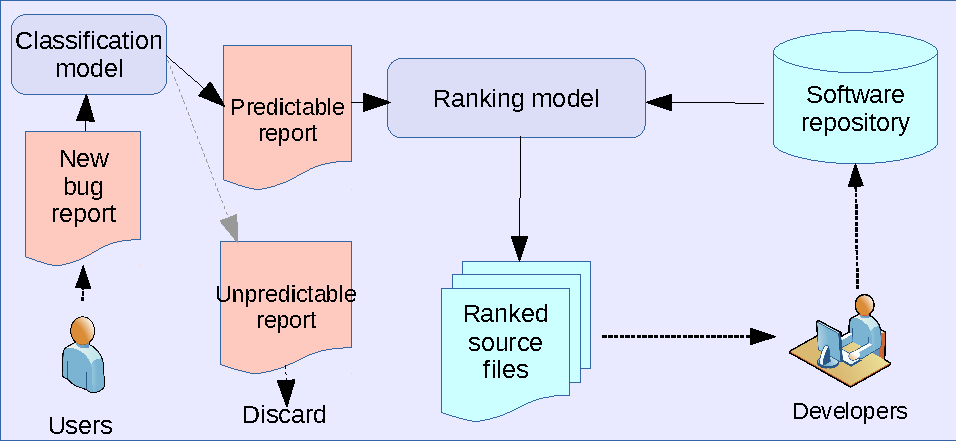
\includegraphics[width=\columnwidth]{figures/prefiltering.pdf}
\caption{High level architecture: pre-filtering before ranking.}
\label{fig:prefiltering architecture}
\end{figure}
Figure~\ref{fig:prefiltering architecture} shows the high level architecture of our bug report pre-filtering approach. When a new bug report is received, it will first be classified by a classification model into one of the two categories: ``predictable'' and ``unpredictable''. A ``predictable'' report is considered as informative and helpful to an IR-based ranking system for bug locating. It serves as input to the ranking system, which uses the report content to rank all the source code files and recommend the top ranked ones as ``buggy'' to developers to review. An ``unpredictable'' report, instead, is considered unhelpful to the IR-based ranking system and will be discarded. By keeping silent on unhelpful reports, the ranking system can reduce the number of false positives and make the recommendations be more trustworthy.

\section{LSTM-based Bug Report Classification}
\label{sec:lstm-based classification}
asdasdasdasdasdasdasdasdsdasda asd dasd asdasdasdasdasdasdasdasdsdasda asd dasd asdasdasdasdasdasdasdasdsdasda asd dasd asdasdasdasdasdasdasdasdsdasda asd dasd asdasdasdasdasdasdasdasdsdasda asd dasd asdasdasdasdasdasdasdasdsdasda asd dasd asdasdasdasdasdasdasdasdsdasda asd dasd asdasdasdasdasdasdasdasdsdasda asd dasd asdasdasdasdasdasdasdasdsdasda asd dasd asdasdasdasdasdasdasdasdsdasda asd dasd asdasdasdasdasdasdasdasdsdasda asd dasd asdasdasdasdasdasdasdasdsdasda asd dasd asdasdasdasdasdasdasdasdsdasda asd dasd asdasdasdasdasdasdasdasdsdasda asd dasd asdasdasdasdasdasdasdasdsdasda asd dasd asdasdasdasdasdasdasdasdsdasda asd dasd asdasdasdasdasdasdasdasdsdasda asd dasd asdasdasdasdasdasdasdasdsdasda asd dasd asdasdasdasdasdasdasdasdsdasda asd dasd asdasdasdasdasdasdasdasdsdasda asd dasd asdasdasdasdasdasdasdasdsdasda asd dasd asdasdasdasdasdasdasdasdsdasda asd dasd asdasdasdasdasdasdasdasdsdasda asd dasd asdasdasdasdasdasdasdasdsdasda asd dasd asdasdasdasdasdasdasdasdsdasda asd dasd asdasdasdasdasdasdasdasdsdasda asd dasd asdasdasdasdasdasdasdasdsdasda asd dasd asdasdasdasdasdasdasdasdsdasda asd dasd 
\begin{figure}[t]
\centering
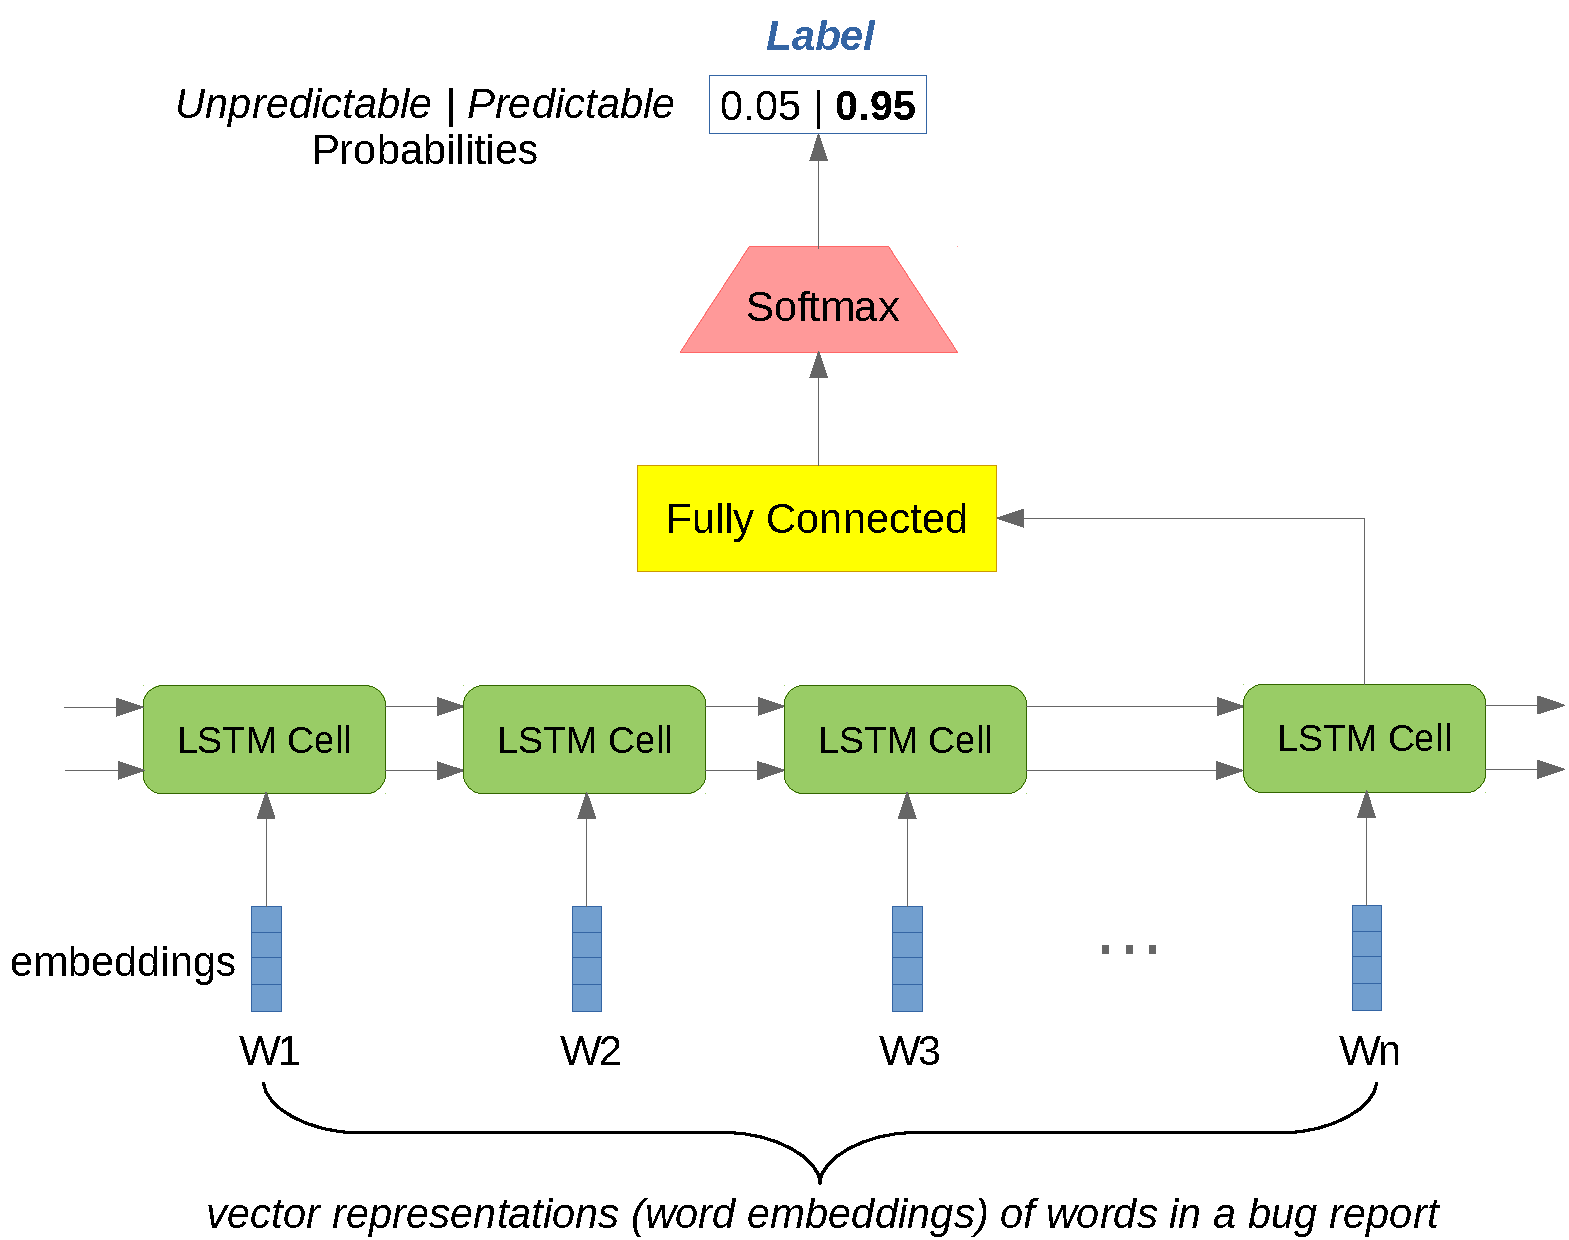
\includegraphics[width=\columnwidth]{figures/lstm.pdf}
\caption{Bug-report classification architecture: using LSTM.}
\label{fig:lstm}
\end{figure}

\begin{figure}[t]
\centering
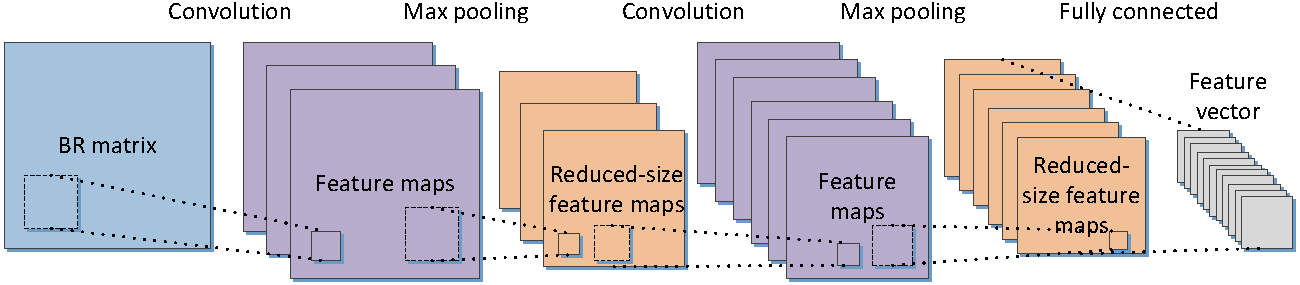
\includegraphics[width=\columnwidth]{figures/cnn.pdf}
\caption{Bug-report classification architecture: using CNN.}
\label{fig:cnn}
\end{figure}



\subsubsection{C.5 Evaluation}
We will evaluate the software defect positioning system on several large-scale open-source projects that contain a sufficient number (more than 2,000) of source code files and previously fixed bug reports. We will conduct experiments on software projects that are written in Java as well as projects written in C/C++ because these programming languages are widely used in both industry and academic. We will use projects from the Eclipse foundation~\footnote{https://eclipse.org/} and Apache foundation~\footnote{https://www.apache.org/} because 1) both have many large-scale open-source projects written in Java and C/C++; 2) the source code packages can be easily downloaded from their GIT repositories; 3) their bug reports or issue reports are public accessible. More specifically, the projects used in our preliminary work \cite{Ye:TSE15} will be used in this study. Additionally, we will run experiments on more projects such as Apache HTTP Server~\footnote{https://httpd.apache.org/} written in C, Lucene~\footnote{https://lucene.apache.org/} (an information retrieval software library) written in Java, and Hadoop~\footnote{http://hadoop.apache.org/} (a software framework for distributed storage and bigdata processing) written in Java. The selection of bug reports for evaluation is based on the same heuristics in \cite{Dallmeier:2007:EBL:1321631.1321702,Ye:FSE14}.

We will run the system to rank all the source code files for a given bug report and compare the result with the actual fix. The evaluation metrics such as \textit{Mean Average Precision} (MAP) \cite{Manning:2008:IIR:1394399} used in our preliminary work \cite{Ye:TSE15} will also be used in this study. Additionally, we will use Normalized Discounted Cumulative Gain (NDCG) \cite{Jarvelin:2002:CGE:582415.582418}, which is widely used in evaluating information retrieval models e.g. web search engines, to evaluate our system.

The PI is aware that user study is an effective way to evaluate the effectiveness of the proposed system in developers' real work. However, this is not the main goal of the proposed study. So the PI leave this to future work after the system is published. This study will also provide the basis for our future research on evaluating the effectiveness and usability of the proposed system in assisting teaching software engineering course at CSUSM.

\subsection{D. Work Plan}
The PI plan to hire one graduate student enrolled in the Master of Science Program in Computer Science (CS) and one undergraduate student enrolled in the Bachelor of Science in Computer Science program at CSUSM to help develop the system. The PI takes the overall responsibility of directing the project and keeps mentoring the students during the development.

\textbf{In the first year}, the graduate student will help implement the bug-report classification model, the LSTM-based semantic similarity feature, and the ranking model running on the server-side. The undergraduate student will implement the client-side programs and the web server that takes charge of the communication between the ranking model and the client-program. Since the ranking model, the database, and the web server work closely, the students will also work together closely during the development.

\textbf{In the second year}, two students will take charge of the maintenance and improvement of the system. Additionally, the graduate student will help run experiments to evaluate the ranking performance of the system on several open-source software projects, analyze the results, and improve the system accordingly. The undergraduate student will help develop a supplemental 3-D VR software visualization module. By the end of this year, the practical system will be published.

\textbf{Recruitment of students} will begin in spring, about three months before they start to work on the project. The PI will broadcast a hiring advertisement on CS-major electronic mailing lists, post a flier on class forums, and make a presentation of the project in the college-wide Frontiers in Science talk. In the coming 2017-2018 academic year, the CS department at CSUSM has a total of 866 undergraduate enrollments and a total of 39 graduate enrollments. Many students have desire to gain hands-on experience by working with faculty members on research projects. The PI will interview interested students. Preference will be given to economically-disadvantaged students, minority students, students making good progress toward their degree, and students who have demonstrated interest in this project.

\subsection{E. Broader Impacts}
The proposed study will result in a practical software system that alleviates develops' effort in bug finding and improves productivity. The system will be published. Any software developers can use and test it on their own projects. The system will be used in the software engineering courses at CSUSM to help students learn software engineering concepts in a lively manner. This project will expose students to an up-to-date software engineering research topic as well as some cutting-edge techniques including artificial neural networks and virtual reality.

The research outcome of this project will provide the basis for the PI's future research in performing user study and collecting user feedback to evaluate the effectiveness of the system in both academic and industry. The experience learned from this project will be very helpful for PI's research in code recommendation and automatic programming. The methodology and techniques used in this project will contribute to the software engineering research community.

The PI graduated with a Ph.D. degree from Ohio University at May 2016 and joined the CS department at CSUSM as an tenure-track faculty at August 2016. The funding to the proposed study will help the PI obtain important computing resources for building a software engineering (SE) research lab at CSUSM to continue his research. This fund, which supports two student assistants, will also help the PI found an SE research group at CSUSM. The research group will work on adapting new techniques to solve SE tasks, applying up-to-date SE research outcome to assist teaching SE courses, and engaging students in doing SE research projects.

The funding will have a significant impact on the quality of education for students here at CSUSM. The funds requested for student assistants will allow some of our economically-disadvantaged students, may of whom work in retail and on campus dining, to have paid positions during the academic year and summer.

Furthermore, funding of the proposed research program will create new opportunities for our students that have strong desire to participate in research projects. The research opportunities created from the funding of the proposed research will directly contribute to providing talented undergraduates at CSUSM with the research experience necessary to be competitive applicants for top-tier Ph.D. programs.

\begin{acks}
  The authors would like to thank Dr. Yuhua Li for providing the
  MATLAB code of the \textit{BEPS} method.

  The authors would also like to thank the anonymous referees for
  their valuable comments and helpful suggestions. The work is
  supported by the \grantsponsor{GS501100001809}{National Natural
    Science Foundation of
    China}{http://dx.doi.org/10.13039/501100001809} under Grant
  No.:~\grantnum{GS501100001809}{61273304}
  and~\grantnum[http://www.nnsf.cn/youngscientists]{GS501100001809}{Young
    Scientists' Support Program}.

\end{acks}
